\documentclass{beamer}
\usepackage[UTF8]{ctex}
\usepackage{hyperref}
\usepackage{graphicx}

\title{C语言程序设计游戏项目}

\author{程渝峰\thanks{Your mailbox} 李梓勤\thanks{tiger1218@foxmail.com}}
\institute{四川大学网络空间安全学院}
\date{\today}

\begin{document}
\begin{frame}
    \titlepage
\end{frame}

\begin{frame}
    \centering
    \Large Welcome to our \href{https://github.com/SCUGamers/Murderer}{Github Repo} to view the game's source code!
\end{frame}

\begin{frame}
    该项目采用了C语言的OpenGL图形库和第三方的对图形进行操作库,实现了 一个2D平台跳跃游戏。该项目的功能包括:
    \begin{enumerate}
        \item 人物左右移动以及跳跃
        \item 人物用剑向前攻击,以及反弹敌人的子弹
        \item 敌人的自动移动以及攻击
        \item 来自环境的特殊效果
    \end{enumerate}

\end{frame}

\begin{frame}
    \begin{figure}[h]
        \centering
        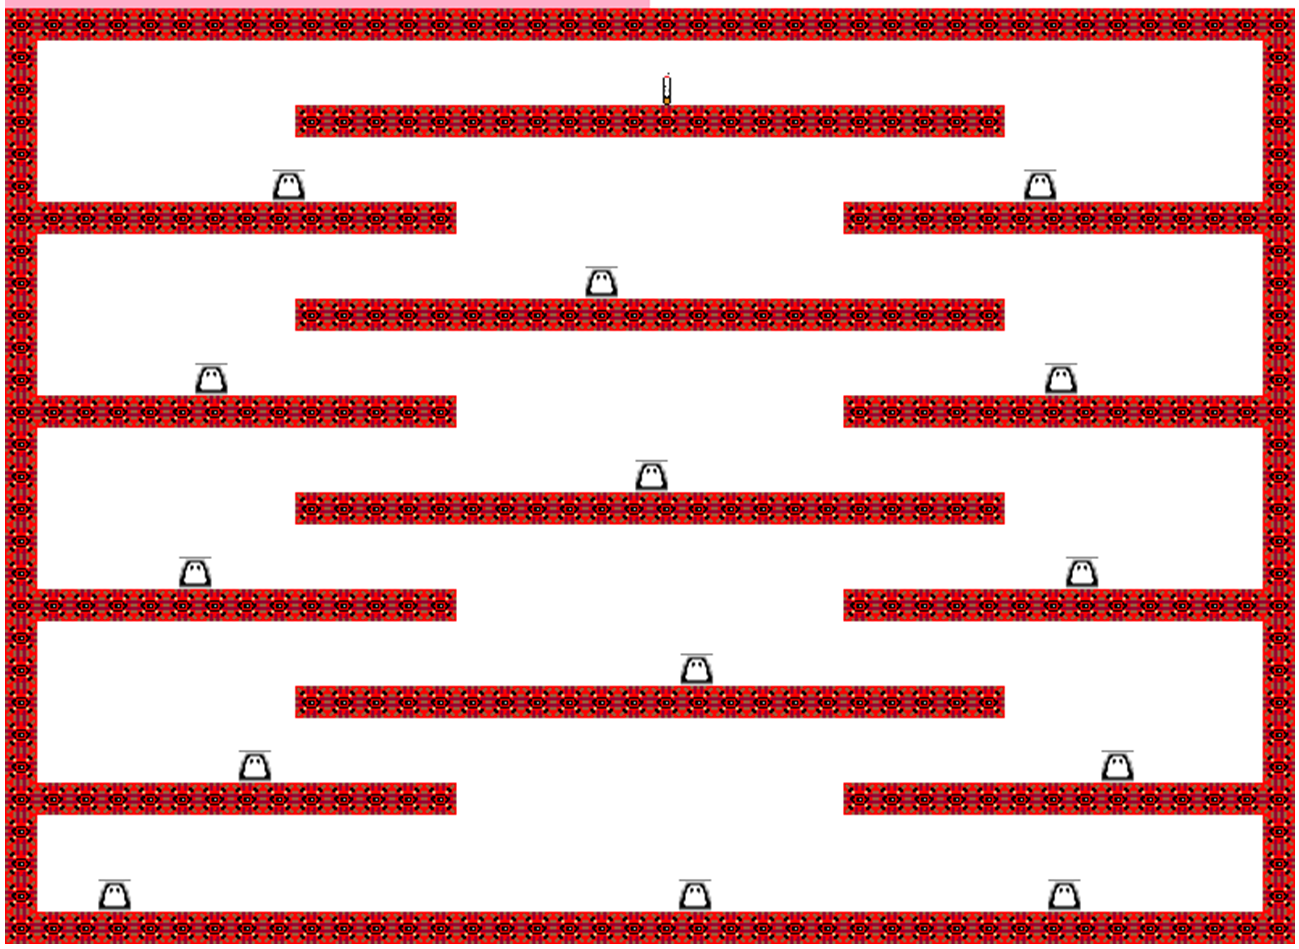
\includegraphics[width=1\textwidth]{img/main_interface}
        \caption{游戏主界面}
    \end{figure}
\end{frame}

\begin{frame}
    \begin{figure}[h]
        \centering
        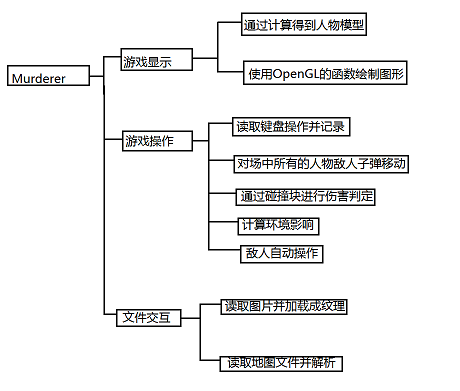
\includegraphics[width=0.8\textwidth]{img/modules}
        \caption{程序的模块划分图}
    \end{figure}
\end{frame}

\begin{frame}
    \begin{figure}[h]
        \centering
        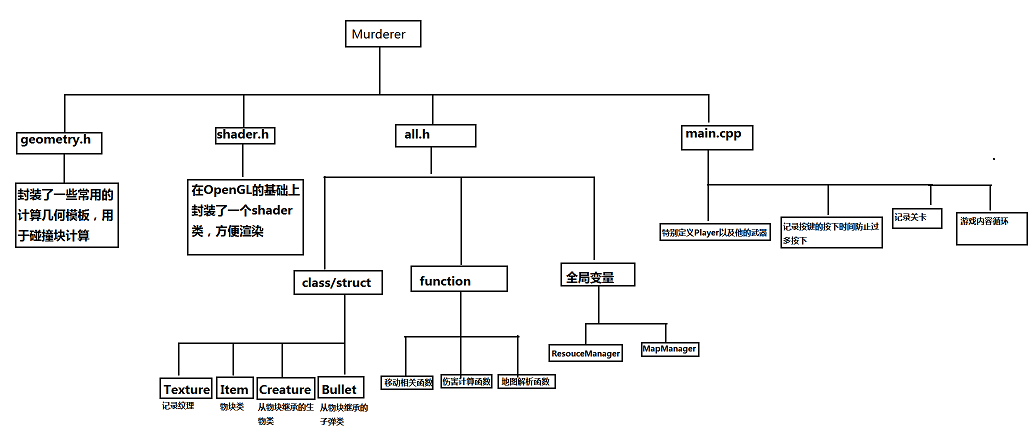
\includegraphics[width=1.1\textwidth]{img/structure}
        \caption{程序的结构图}
    \end{figure}
\end{frame}

\begin{frame}
    \begin{figure}[h]
        \centering
        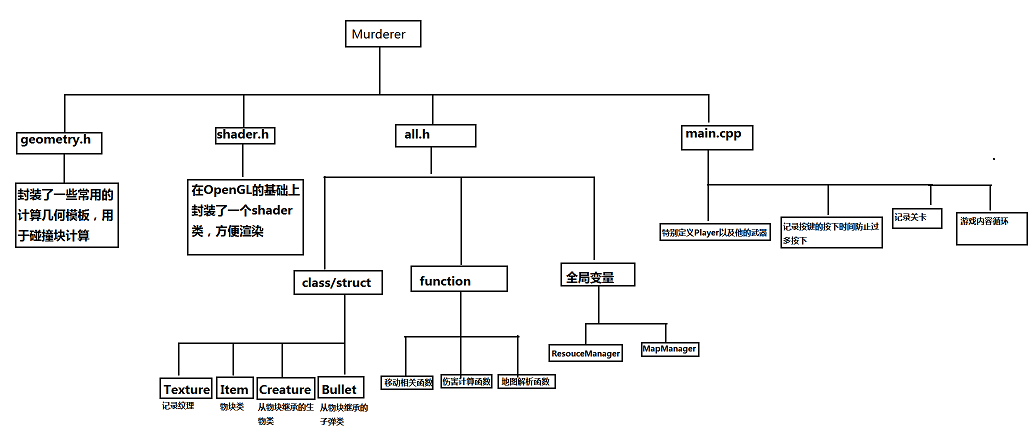
\includegraphics[width=1.1\textwidth]{img/structure}
        \caption{程序的结构图}
    \end{figure}
\end{frame}

\end{document}